\chapter{Detalles de Implementación y Experimentos}\label{chapter:implementation}


\section{Implementación}

\subsection{Estructura del proyecto}

El sistema propuesto utiliza dos repositorios: el primero se encarga de definir el backend que gestiona los endpoints; el segundo para la construcción del contrato inteligente que refleje la lógica de las transacciones hechas a la blockchain que contiene los certificados.

El backend, encargado de procesar los endpoints y obtener las respuestas pertinentes, está modularizado a grandes rasgos de la siguiente forma:
\begin{itemize}
	\item \textbf{api}: Esta carpeta define cuales son los endpoints que existen en el sistema
	\item \textbf{services}: Directorio que contiene los servicios usados por los endpoints para computar la respuesta.
	\item \textbf{repo}: Contiene la lógica para comunicarse con las bases de datos y garantizar la persistencia de estos.
	\item \textbf{schema}: Carpeta que contiene las estructuras que representan información. Entre ellos están los modelos, los dto(objetos de transferencia de datos) y las constantes usadas en el proyecto. Además están definidas las funciones `mapper' que saben como convertir estructuras de un tipo a otro.
	\item \textbf{lib}: Directorio donde están funcionalidades menores de uso común.
	\item \textbf{main.go}: Archivo encargado de cargar la aplicación. En él se adjuntan las librerías principales.
\end{itemize}

Por otro lado existen dos contratos inteligentes que permiten gestionar los certificados. El primero es `Certificacates' y es para realizar las operaciones CRUD: creación, lectura básica, modificación, y eliminación. El segundo es `Common', un contrato generalizado para cualquier activo, no solo certificados. En él está definida la lógica para realizar consultas enriquecidas, dichas consultas enriquecidas permiten buscar los datos en la blockchain aplicando condiciones a las propiedades de los activos. Además, el contrato `Common' facilita obtener el historial de modificaciones aplicadas a los datos.

\subsection{Endpoints}
Se ha mencionado ya, que se utiliza Iris como framework para desarrollar la estructura web. Iris permite inyectar dependencias a los endpoints que lo requieran, obteniendo así una optimización en el uso de los recursos. Para inyectar dichas dependencias se registran al principio de la función [\ref{code:1}]. Luego iris se encargará de entregarlas automáticamente a las funciones que describen los endpoints.

Para definir las rutas de acceso se crean Grupos(Party). Estos grupos se pueden anidar par representar funcionalidades comunes. Los endpoints se crean especificando el método que debe tener la petición, su subruta y la función de Go que se encargará de procesarlo.

\begin{lstlisting}[language=Go,caption={Sistema de rutas de Iris}, label={code:1}]
// Register dependencies	
hero.Register(depObtainUserCred)
hero.Register(lib.DepObtainUserDid)
hero.Register(svcAuth)
hero.Register(svcUser)
hero.Register(repoUser)

// Simple group: v1
v1 := app.Party("/api/v1")
{
	// registering unprotected router
	authRouter := v1.Party("/auth") // authorize
	{
		// --- REGISTERING ENDPOINTS ---
		authRouter.Post("/", hero.Handler(h.authIntent))
	}
	
	// registering protected router
	guardAuthRouter := v1.Party("/auth")
	{
		// --- GROUP / PARTY MIDDLEWARES ---
		guardAuthRouter.Use(*mdwAuthChecker) // registering access token checker middleware
		
		// --- REGISTERING ENDPOINTS ---
		guardAuthRouter.Get("/logout", h.logout)
		guardAuthRouter.Get("/profile", hero.Handler(h.getUserProfile))
	}
\end{lstlisting}

Se puede observar en \ref{code:1} que existen dos party comunes con la misma ruta. La diferencia está en que en uno de ellos se especifica el uso de los tokens de acceso. Esta es la implementación de la idea de exponer ciertas funciones al uso público y otras solo para usuarios registrados.

En el presente sistema se usa Swagger para documentar los endpoints. Swagger permite definir la estructura de la entrada esperada por estas funciones a la par que su salida. Deja conocer también los distintos tipos de respuestas que se pueden devolver. Además se define la estructura que tendrá la ruta para acceder al endpoint. Esta información extra se sitúa como comentario encima de la función que se desee documentar [\ref{code:2}].
\begin{lstlisting}[language=Go,caption={Endpoint para obtener los datos del usuario actualmente autenticado}, label={code:2}]
// getUserProfile Get user from the BD.
// @Summary Get user
// @Tags Auth
// @Security ApiKeyAuth
// @Produce  json
// @Param Authorization header string true "Insert access token" default(Bearer <Add access token here>)
// @Success 200 {object} dto.UserResponse "OK"
// @Failure 401 {object} dto.Problem "err.unauthorized"
// @Failure 500 {object} dto.Problem "err.generic
// @Router /auth/profile [get]
func (h HAuth) getUserProfile(ctx iris.Context, params dto.InjectedParam, service service.ISvcUser) {
	user, problem := service.GetUserByUsernameSvc(params.Username)
	if problem != nil {
		(*h.response).ResErr(problem, &ctx)
		return
	}
	h.response.ResOKWithData(user, &ctx)
}
\end{lstlisting}

En \ref{code:2} se observa como los endpoints solo capturan los datos que pasan y generan las respuestas con los resultados. El proceso de computar esa respuesta es responsabilidad de los servicios.

\subsection{Servicios}
Los servicios son los encargados de computar los datos que serán devueltos al usuario como respuesta a su petición [\ref{code:3}]. Es común que tengan que consultar datos que están almacenados en el nivel de persistencia, pero la lógica para obtenerlos no está escrita en ellos. Los datos que se almacenan en el nivel de persistencia pueden tener información que solo tenga sentido para el sistema. En estos casos se usan los dto y es común ver los llamados a funciones mapper para convertir lo devuelto por la capa de persistencia en objetos que representen esos datos de manera amistosa al usuario.

\begin{lstlisting}[language=Go,caption={Servicio para obtener los usuarios de la base de datos}, label={code:3}]
func (s *svcUser) GetUsersSvc(pagination *dto.Pagination) (*dto.Pagination, *dto.Problem) {
	res, err := (*s.repoUser).GetUsers(pagination)
	if err != nil {
		return nil, lib.NewProblem(iris.StatusExpectationFailed, schema.ErrBuntdb, err.Error())
	}
	var usersResponse []dto.UserResponse
	items := res.Rows.([]models.User)
	for i := 0; i < len(items); i++ {
		usersResponse = append(usersResponse, mapper.MapModelUser2DtoUserResponse(items[i]))
	}
	res.Rows = usersResponse
	return res, nil
}
\end{lstlisting}

Como parte de la seguridad de la propuesta se enunció que no se almacenarían contraseñas en las bases de datos, sino el resultado de aplicarles una función de hash. Es precisamente en los servicios donde se implementa esta lógica [\ref{code:4}]

\begin{lstlisting}[language=Go,caption={Servicio para crear un usuario}, label={code:4}]
func (s *svcUser) PostUserSvc(user dto.UserData) (dto.UserResponse, *dto.Problem) {
	passphraseEncoded, _ := lib.Checksum("SHA256", []byte(user.Passphrase))
	user.Passphrase = passphraseEncoded
	modelUser := mapper.MapUserData2ModelUser(0, user)
	resUser, err := s.repoUser.AddUser(modelUser)
	if err != nil {
		return dto.UserResponse{}, lib.NewProblem(iris.StatusExpectationFailed, schema.ErrBuntdb, err.Error())
	}
	return mapper.MapModelUser2DtoUserResponse(resUser), nil
}
\end{lstlisting}

\subsection{Repos}
Los repos son donde está definida la capa de comunicación entre el sistema y las bases de datos usadas. Aquí es donde se implementa la lógica para la obtención de esos datos. La base de datos que garantiza la persistencia de los certificados es una blockchain por lo que se necesita un puente entre ambos sistemas. La base de datos de los usuarios no tiene que ejecutarse necesariamente en la misma computadora. El sistema brinda la facilidad de crear un servicio en cualquier otro lugar con esa BD y realizar la comunicación con el, por tanto un comunicación es requerida.

En el caso de la base de datos de usuarios se utiliza PostgreSQL y la ORM (Object Relational Mapping) es Gorm. Gorm permite realizar las operaciones CRUD pero no tiene un sistema de paginado implementado. Por esto, el proceso de paginado para grandes listas se realiza dentro esta componente puente [\ref{code:5}]. La implementación de las demás funciones es similar a esta, salvo el uso de la función de Gorm correspondiente(create, save, first, etc) [\ref{code:6}]

\begin{lstlisting}[language=Go,caption={Función que consulta los usuarios}, label={code:5}]
// GetUsers return a list of dto.User
func (r *RepoUser) GetUsers(pagination *dto.Pagination) (*dto.Pagination, error) {
	var users []models.User
	result := r.DB.Scopes(paginate(users, pagination, r.DB)).Find(&users)
	if result.Error != nil {
		return &dto.Pagination{}, result.Error
	}
	pagination.Rows = users
	return pagination, nil
}
\end{lstlisting}

\begin{lstlisting}[language=Go,caption={Función para modificar un usuario}, label={code:6}]
// UpdateUser Update user with id UserID to new data in database
// Returns nil if user was updated correctly, otherwise return error found
func (r *RepoUser) UpdateUser(userID int, user models.User) (models.User, error) {
	var userInDB models.User
	if result := r.DB.First(&userInDB, userID); result.Error != nil {
		return models.User{}, result.Error
	}
	result := r.DB.Save(&user)
	return user, result.Error
}
\end{lstlisting}

Para comunicarse con la blockchain, se utilizan dos funciones: query e invoke. Las transacciones que sean de tipo query no modifican el estado de la blockchain mientras que las invoke si. Contenida en estas transacciones está la función del chaincode que desea ser ejecutada y en el payload todos los argumentos que necesita.

\subsection{Schema}
Los usuarios cumplen el modelo [\ref{code:7}] y pueden ser transformados a dto como [\ref{code:8}] dependiendo de la información que quiera ser obtenida o proporcionada al usuario. La transformación se realiza a través de funciones mapper como [\ref{code:9}]. Esta función mapper en particular cambia la representación de los roles en la tabla por un texto familiar para el usuario. Ambas representaciones: modelos y dtos pueden contener la forma de representación que tendrán en json, en algunos casos se utiliza la biblioteca Validator V10 para especificar validaciones para cada campo. Este mismo patrón de modelo, dto y mapper es seguido para trabajar las representaciones de los certificados.

\begin{lstlisting}[language=Go,caption={Modelo de usuarios}, label={code:7}]
type User struct {
	ID         int    `json:"id" gorm:"primaryKey"`
	Username   string `json:"username" gorm:"uniqueIndex" validate:"required"`
	Passphrase string `json:"passphrase" validate:"required"`
	FirstName  string `json:"firstname" validate:"required"`
	LastName   string `json:"lastname" validate:"required"`
	Email      string `json:"email" validate:"required,email"`
	Role       string `json:"rol_id" validate:"required"`
}
\end{lstlisting}

\begin{lstlisting}[language=Go,caption={DTO UserResponse, encargado de presentar los detalles sobre usuarios de la base de datos}, label={code:8}]
type UserResponse struct {
	ID        int    `json:"id"`
	Username  string `json:"username" validate:"required"`
	FirstName string `json:"firstname" validate:"required"`
	LastName  string `json:"lastname" validate:"required"`
	Email     string `json:"email" validate:"required,email"`
	Role      string `json:"rol" validate:"required"`
}
\end{lstlisting}

\begin{lstlisting}[language=Go,caption={Mapper de modelo de usuario a dto de usuarios para mostrar al cliente}, label={code:9}]
func MapModelUser2DtoUserResponse(user models.User) dto.UserResponse {
	return dto.UserResponse{
		ID:        user.ID,
		Username:  user.Username,
		FirstName: user.FirstName,
		LastName:  user.LastName,
		Email:     user.Email,
		Role:      roleLabel2RoleName(user.Role),
	}
}
\end{lstlisting}

\subsection{Contrato Inteligente de certificados}
En los contratos inteligentes está la lógica de la interacción con la blockchain. Una función interesante y que vale la pena analizar es la de modificar un activo(certificado). Dado que la modificación es de manera libre interesa comprobar que se mantenga la consistencia de los activos. Los comentarios en [\ref{code:10}] explican la idea para mantener dicha congruencia.

\begin{lstlisting}[language=Go,caption={Función para modificar un certificado de la blockchain}, label={code:10}]
// UpdateAsset updates an existing asset in the world state with provided parameters.
func (s *ContractCertificate) UpdateAsset(ctx contractapi.TransactionContextInterface, request *Asset) error {
	composeKey, assetJSON, err := lus.ExistsAssetFromId(ctx.GetStub(), lus.CodCert, request.ID)
	if err != nil {
		return err
	} else if assetJSON == nil {
		return fmt.Errorf(lus.ErrorNotExistInState, request.ID)
	}
	// Check new params of the asset consistency
	
	// If certificate is valid then it should have the 3 signatures
	if (request.Status == Valid) && (request.SecretaryValidating == "" || request.DeanValidating == "" || request.RectorValidating == "") {
		return fmt.Errorf(lus.ErrorInconsistentStatus)
	}
	// If certificate is SignedSD then it should have Secretary and Dean signatures
	if (request.Status == SignedSD) && (request.SecretaryValidating == "" || request.DeanValidating == "") {
		return fmt.Errorf(lus.ErrorInconsistentStatus)
	}
	// If certificate is SignedSD then it should have Secretary and Dean signatures
	if (request.Status == SignedS) && (request.SecretaryValidating == "") {
		return fmt.Errorf(lus.ErrorInconsistentStatus)
	}
	// If certificate is revoked then it should have a revoked reason
	if (request.Status == Invalid) && (request.InvalidReason == "") {
		return fmt.Errorf(lus.ErrorInconsistentInvalidation)
	}
	// overwritting original asset with new asset
	asset := Asset{
		DocType:               lus.CodCert,
		ID:                    request.ID,
		Certification:         request.Certification,
		GoldCertificate:       request.GoldCertificate,
		Emitter:               request.Emitter,
		Accredited:            request.Accredited,
		Date:                  request.Date,
		CreatedBy:             request.CreatedBy,
		SecretaryValidating:   request.SecretaryValidating,
		DeanValidating:        request.DeanValidating,
		RectorValidating:      request.RectorValidating,
		FacultyVolumeFolio:    request.FacultyVolumeFolio,
		UniversityVolumeFolio: request.UniversityVolumeFolio,
		InvalidReason:         request.InvalidReason,
		Status:                request.Status,
	}
	
	assetJSON, err = json.Marshal(asset)
	if err != nil {
		return err
	}
	
	return ctx.GetStub().PutState(composeKey, assetJSON)
}
\end{lstlisting}

Para realizar consultas sobre los archivos de manera que se cumplan ciertas condiciones sobre sus propiedades existen las consultas enriquecidas [\ref{code:11}]. Para este tipo de consultas debe ser especificado un selector, dicho selector no es más que una estructura especial que contiene definidas dichas condiciones. La lista de certificados que cumplan el criterio puede ser paginados usando las propiedades `pageLimit' y `bookmark'. Estas propiedades expresan el límite de activos que serán devueltos y un identificador para saber por cual activo empezar a devolver. Este `bookmark' es entregado como parte de la respuesta a la consulta, si se desea seguir mostrando certificados a partir del último visto entonces puede pasarse este valor.

\begin{lstlisting}[language=Go,caption={Código del archivo App.vue}, label={code:11}]
// QueryAssetsWithPagination uses a query string, page size and a bookmark to perform a query
// for assets. Query string matching state database syntax is passed in and executed as is.
// The number of fetched records would be equal to or lesser than the specified page size.
// Supports ad hoc queries that can be defined at runtime by the client.
// If this is not desired, follow the QueryAssetsForOwner example for parameterized queries.
// Only available on state databases that support rich query (e.g. CouchDB)
// Paginated queries are only valid for read only transactions.
// Example: Pagination with Ad hoc Rich Query
func (cc *ContractCommon) QueryAssetsWithPagination(ctx contractapi.TransactionContextInterface, request lus.RichQuerySelector) (*lus.PaginatedQueryResponse, error) {
	queryString, err := json.MarshalToString(request.QueryString)
	if err != nil {
		return nil, err
	} else if queryString == "" {
		return nil, fmt.Errorf("missing query string")
	}
	
	return lus.GetQueryResultForQueryStringWithPagination(ctx, queryString, int32(request.PageSize), request.Bookmark)
}
\end{lstlisting}

\section{Experimentos de Rendimiento}

La implementación del sistema de certificaciones de estudiantes basadas en blockchain se evaluó utilizando dos métricas de rendimiento principales: el tiempo promedio que se tarda en emitir un certificado y el tiempo de latencia, medidos ambos en segundos. La latencia se refiere al tiempo que tarda la red blockchain en procesar la transacción. El sistema de certificación electrónica implementado con Hyperledger Fabric se probó en 1000 transacciones para emitir 1000 certificados de estudiantes. El tiempo computacional promedio de implementación de la certificación se muestra en la tabla \ref{tab:1}.

\begin{table}[!h]
	\caption{Resultados de realizar 1000 transacciones}
	\label{tab:1}
	\begin{tabular}{ll} \toprule
		\textbf{Medición} & \textbf{Tiempo medio en segundos} \\ \midrule
		Emitir Certificado & 2.1 (Hasta que se confirma la adición)  \\
		Tiempo de Latencia & 1.5 (Obteniendo certificados por acreditado)  \\ \bottomrule
	\end{tabular}
\end{table}

Otra métrica de rendimiento se obtiene comprobando la relación entre la cantidad de transacciones simultaneas realizadas y el tiempo que le toma cumplirlas. Para comprobarlo se generaron de manera aleatoria transacciones y se ejecutaron para realizar la medición. Se realizó este proceso 7 veces: Primero con 500 transacciones, luego 1000, 1500, 2000, 2500, 3000 y 3500. Cuando se unen los puntos ploteados se genera la gráfica \ref{fig:13}

\begin{figure}[h!]
	\centering
	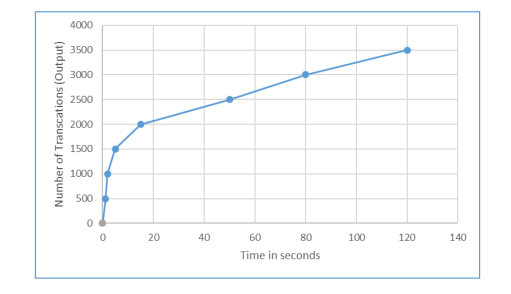
\includegraphics[width=\linewidth]{Graphics/plot.png}
	\caption{Tiempo que toma realizar n transacciones simultáneas}
	\label{fig:13}
\end{figure}

Es asumible por la observación que el tiempo requerido para cumplir con las solicitudes de transacciones aumenta exponencialmente a medida que aumenta la cantidad de transacciones simultáneas.

Se mencionó durante la introducción que el sistema propuesto en este documento tiene un complemento. Existe un trabajo titulado ``Interfaz de usuario para un Gestor de Certificados Académicos'' cuya solución se enlaza directamente a los endpoints que implementan la lógica aquí expuesta. En ese trabajo ser realizan una serie de pruebas sobre la integridad de los endpoints. Se alterar los datos almacenados para intentar encontrar inconsistencias. Se prueba la efectividad del sistema de control de acceso a funcionalidades restringidas. Se envian peticiones para crear o modificar los datos con campos vacíos, entre otras pruebas. Todos los test ejecutados allí tuvieron una respuesta correcta.